%%%%%%%%%%%%%%%%%%%%% chapter.tex %%%%%%%%%%%%%%%%%%%%%%%%%%%%%%%%%
%
% sample chapter
%
% Use this file as a template for your own input.
%
%%%%%%%%%%%%%%%%%%%%%%%% Springer-Verlag %%%%%%%%%%%%%%%%%%%%%%%%%%
%\motto{Use the template \emph{chapter.tex} to style the various elements of your chapter content.}

\chapter{Rosetta Code Tasks starting with I}

\section*{IPC via named pipe}

\href{http://en.wikipedia.org/wiki/Named\_pipe}{Named pipe}, or FIFO, is
a way of providing inter-process communications (IPC). To demonstrate
how it works, create two pipes, say, ``in'' and ``out'' (choose suitable
names for your system), and write a program that works the two pipes
such that:

\begin{enumerate}
\item
  Data written to the ``in'' FIFO will be discarded except the byte
  count, which will be added to a total tally kept by the program;
\item
  Whenever another process reads the ``out'' FIFO, it should receive the
  total count so far.
\end{enumerate}

Possible issues:

\begin{itemize}
\item
  Chances are you don't already have ``in'' and ``out'' pipes lying
  around. Create them within your program or without, at your
  discretion. You may assume they are already created for you.
\item
  Your program may assume it's the sole reader on ``in'' and the sole
  writer on ``out''.
\item
  Read/write operations on pipes are generally
  \href{http://en.wikipedia.org/wiki/Blocking\_(computing)}{blocking}.
  Make your program responsive to both pipes, so that it won't block
  trying to read the ``in'' pipe while leaving another process hanging
  on the other end of ``out'' pipe indefinitely -- or vice versa. You
  probably need to either poll the pipes or use multi-threading.
\item
  You may assume other processes using the pipes behave; specificially,
  your program may assume the process at the other end of a pipe will
  not unexpectedly break away before you finish reading or writing.
\end{itemize}



\begin{wideverbatim}

(call 'mkfifo "in" "out")              # Create pipes

(zero *Cnt)                            # Initialize byte counter

(unless (fork)                         # Handle "out" pipe
   (loop
      (out "out"
         (sync)
         (tell)
         (prinl *Cnt) ) ) )

(unless (fork)                         # Handle "in" pipe
   (let P (open "in")
      (loop
         (in P                         # Open twice, to avoid broken pipes
            (while (rd 1)                 # (works on Linux, perhaps not POSIX)
               (tell 'inc ''*Cnt) ) ) ) ) )

(push '*Bye '(call 'rm "in" "out"))    # Remove pipes upon exit
(wait)                                 # (Terminate with Ctrl-C)

Test:

\$ line <out
0
\$ echo abc >in
\$ line <out
4
\$ echo äöü >in
\$ line <out
11

\end{wideverbatim}

\pagebreak{}
\section*{Identity matrix}

Build an \href{http://en.wikipedia.org/wiki/identity\_matrix}{identity
matrix} of a size known at runtime. An identity matrix is a square
matrix, of size \emph{n} × \emph{n}, where the diagonal elements are all
1s, and the other elements are all 0s.

\begin{figure}[H]
\centering
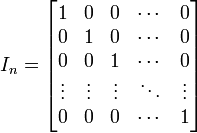
\includegraphics[scale=.6]{graphics/fe1a9857fd0a471baec6c538220e1bc9.png}
% \caption{I\_n = \textbackslash{}begin\{bmatrix\} 1 \& 0 \& 0 \&
% \textbackslash{}cdots \& 0 \textbackslash{}\textbackslash{} 0 \& 1 \& 0
% \& \textbackslash{}cdots \& 0 \textbackslash{}\textbackslash{} 0 \& 0 \&
% 1 \& \textbackslash{}cdots \& 0 \textbackslash{}\textbackslash{}
% \textbackslash{}vdots \& \textbackslash{}vdots \& \textbackslash{}vdots
% \& \textbackslash{}ddots \& \textbackslash{}vdots
% \textbackslash{}\textbackslash{} 0 \& 0 \& 0 \& \textbackslash{}cdots \&
% 1 \textbackslash{}\textbackslash{} \textbackslash{}end\{bmatrix\}}
\end{figure}

\begin{wideverbatim}

(de identity (Size)
   (let L (need Size (1) 0)
      (make
         (do Size
            (link (copy (rot L))) ) ) ) )

Test:

: (identity 3)
-> ((1 0 0) (0 1 0) (0 0 1))

: (mapc println (identity 5))
(1 0 0 0 0)
(0 1 0 0 0)
(0 0 1 0 0)
(0 0 0 1 0)
(0 0 0 0 1)

\end{wideverbatim}

\pagebreak{}
\section*{Image convolution}

One class of image digital filters is described by a rectangular matrix
of real coefficients called \textbf{kernel} convoluted in a sliding
window of image pixels. Usually the kernel is square
\emph{K}\textsubscript{\emph{k}\emph{l}}, where \emph{k}, \emph{l} are
in the range -\emph{R},-\emph{R}+1,..,\emph{R}-1,\emph{R}.
\emph{W}=2\emph{R}+1 is the kernel width. The filter determines the new
value of a monochromatic image pixel P\textsubscript{\emph{ij}} as a
convolution of the image pixels in the window centered in \emph{i},
\emph{j} and the kernel values:

\begin{figure}[H]
\centering
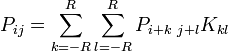
\includegraphics[scale=.6]{graphics/058aad0ea1d9f900745a1e688b75cec8.png}
\end{figure}

Color images are usually split into the channels which are filtered
independently. A color model can be changed as well, i.e. filtration
is performed not necessarily in RGB. Common kernels sizes are 3x3 and
5x5. The complexity of filtrating grows quadratically
(\emph{O}(\emph{n}\textsuperscript{2})) with the kernel width.

\textbf{Task}: Write a generic convolution 3x3 kernel filter. Optionally
show some end user filters that use this generic one.

\emph{(You can use, to test the functions below, these \emph{input}
  and \emph{output} solutions.)}



\begin{wideverbatim}

(scl 3)

(de ppmConvolution (Ppm Kernel)
   (let (Len (length (car Kernel))  Radius (/ Len 2))
      (make
         (chain (head Radius Ppm))
         (for (Y Ppm  T  (cdr Y))
            (NIL (nth Y Len)
               (chain (tail Radius Y)) )
            (link
               (make
                  (chain (head Radius (get Y (inc Radius))))
                  (for (X (head Len Y) T)
                     (NIL (nth X 1 Len)
                        (chain (tail Radius (get X (inc Radius)))) )
                     (link
                        (make
                           (for C 3
                              (let Val 0
                                 (for K Len
                                    (for L Len
                                       (inc 'Val
                                          (* (get X K L C) (get Kernel K L)) ) ) )
                                 (link (min 255 (max 0 (*/ Val 1.0)))) ) ) ) )
                     (map pop X) ) ) ) ) ) ) )

Test using 'ppmRead' from [[Bitmap/Read a PPM file#PicoLisp]] and 'ppmWrite'
from [[Bitmap/Write a PPM file#PicoLisp]]:

# Sharpen
(ppmWrite
   (ppmConvolution
      (ppmRead "Lenna100.ppm")
      '((-1.0 -1.0 -1.0) (-1.0 +9.0 -1.0) (-1.0 -1.0 -1.0)) )
   "a.ppm" )

# Blur
(ppmWrite
   (ppmConvolution
      (ppmRead "Lenna100.ppm")
      '((0.1 0.1 0.1) (0.1 0.1 0.1) (0.1 0.1 0.1)) )
   "b.ppm" )

\end{wideverbatim}

\pagebreak{}
\section*{Image Noise}


Generate a random black and white 320x240 image continuously, showing
FPS (frames per second).

Sample image:

\begin{figure}[H]
\centering

\includegraphics[scale=.6]{graphics/NoiseOutput.png}
\end{figure}

\begin{wideverbatim}

This solution works on ErsatzLisp, the Java version of PicoLisp. It creates a
'JFrame' window, and calls inlined Java code to handle the image.

(javac "ImageNoise" "JPanel" NIL
      "java.util.*"
      "java.awt.*" "java.awt.image.*" "javax.swing.*" )
   int DX, DY;
   int[] Pixels;
   MemoryImageSource Source;
   Image Img;
   Random Rnd;

   public ImageNoise(int dx, int dy) {
      DX = dx;
      DY = dy;
      Pixels = new int[DX * DY];
      Source = new MemoryImageSource(DX, DY, Pixels, 0, DX);
      Source.setAnimated(true);
      Img = createImage(Source);
      Rnd = new Random();
   }

   public void paint(Graphics g) {update(g);}
   public void update(Graphics g) {g.drawImage(Img, 0, 0, this);}

   public void draw() {
      for (int i = 0; i < Pixels.length; ++i) {
         int c = Rnd.nextInt(255);
         Pixels[i] = 0xFF000000 | c<<16 | c<<8 | c;
      }
      Source.newPixels();
      paint(getGraphics());
   }
/**/

(de imageNoise (DX DY Fps)
   (let
      (Frame (java "javax.swing.JFrame" T "Image Noise")
         Noise (java "ImageNoise" T DX DY)
         Button (java "javax.swing.JButton" T "OK") )
      (java Frame "add" Noise)
      (java Frame "add" "South" Button)
      (java Button "addActionListener"
         (interface "java.awt.event.ActionListener"
            'actionPerformed '((Ev) (bye)) ) )
      (java Frame "setSize" DX DY)
      (java Frame "setVisible" T)
      (task (/ -1000 Fps) 0
         Image Noise
         (java Image "draw") ) ) )

# Start with 25 frames per second
(imageNoise 320 240 25)

\end{wideverbatim}

\pagebreak{}
\section*{Include a file}

The task is to demonstrate the language's ability to include source code
from other files.

\begin{wideverbatim}

The function '[http://software-lab.de/doc/refL.html#load load]' is used for
recursively executing the contents of files.

(load "file1.l" "file2.l" "file3.l")

\end{wideverbatim}

\pagebreak{}
\section*{Increment a numerical string}

This task is about incrementing a numerical string.

\begin{wideverbatim}

(format (inc (format "123456")))

\end{wideverbatim}

\pagebreak{}
\section*{Infinity}

Write a function which tests if infinity is supported for floating point
numbers (this step should be omitted for languages where the language
specification already demands the existence of infinity, e.g. by
demanding \emph{IEEE} numbers), and if so, returns positive
infinity. Otherwise, return the largest possible positive floating point
number.

For languages with several floating point types, use the type of the
literal constant 1.5 as floating point type.

C.F. \emph{Extreme floating point values}


\begin{wideverbatim}

The symbol '[http://software-lab.de/doc/refT.html#T T]' is used to represent
infinite values, e.g. for the length of circular lists, and is greater than any
other value in comparisons. PicoLisp has only very limited floating point
support (scaled bignum arithmetics), but some functions return 'T' for infinite
results.

(load "@lib/math.l")

: (exp 1000.0)
-> T

\end{wideverbatim}

\pagebreak{}
\section*{Inheritance/Multiple}

Multiple inheritance allows to specify that one \emph{class} is a
subclass of several other classes. Some languages allow multiple
\emph{inheritance} for arbitrary classes, others restrict it to
interfaces, some don't allow it at all.

Write two classes (or interfaces) \texttt{Camera} and
\texttt{MobilePhone}, then write a class \texttt{CameraPhone} which is
both a \texttt{Camera} and a \texttt{MobilePhone}.

There is no need to implement any functions for those classes.

\begin{wideverbatim}

(class +Camera)

(class +MobilePhone)

(class +CameraPhone +Camera +MobilePhone)
(class +Camera)

(class +MobilePhone)

(class +CameraPhone +Camera +MobilePhone)

\end{wideverbatim}

\pagebreak{}
\section*{Inheritance/Single}

\emph{This task is about derived types; for implementation inheritance,
see \emph{Polymorphism}.}

Inheritance is an operation of \emph{type algebra} that creates a new
type from one or several parent types. The obtained type is called
\textbf{derived type}. It inherits some of the properties of its
parent types. Usually inherited properties are:

\begin{itemize}
\item
  methods
\item
  components
\item
  parts of the representation
\end{itemize}

The \emph{class} of the new type is a \textbf{subclass}
of the classes rooted in the parent types. When all (in certain sense)
properties of the parents are preserved by the derived type, it is said
to be a
\href{http://en.wikipedia.org/wiki/Liskov\_substitution\_principle}{Liskov
subtype}. When properties are preserved then the derived type is
\emph{substitutable} for its parents in all contexts. Usually full
substitutability is achievable only in some contexts.

Inheritance is

\begin{itemize}
\item
  \textbf{single}, when only one parent is allowed
\item
  \textbf{\emph{multiple}}, otherwise
\end{itemize}

Some single inheritance languages usually allow multiple inheritance for
certain \emph{abstract types}, interfaces in
particular.

Inheritance can be considered as a relation parent-child. Parent types
are sometimes called \textbf{supertype}, the derived ones are
\textbf{subtype}. This relation is
\href{http://en.wikipedia.org/wiki/Transitive\_relation}{transitive} and
\href{http://en.wikipedia.org/wiki/Reflexive\_relation}{reflexive}.
Types bound by the relation form a
\href{http://en.wikipedia.org/wiki/Directed\_acyclic\_graph\_directed\_acyclic\_graph}{wp:Directed\_acyclic\_graph
directed acyclic graph} (ignoring reflexivity). With single inheritance
it becomes a
\href{http://en.wikipedia.org/wiki/Tree\_(graph\_theory)}{tree}.

\pagebreak{}

\textbf{Task}: Show a tree of types which inherit from each other. The
top of the tree should be a class called Animal. The second level should
have Dog and Cat. Under Dog should be Lab and Collie. None of the
classes need to have any functions, the only thing they need to do is
inherit from the specified superclasses (overriding functions should be
shown in \emph{Polymorphism}). The tree should look
like this:


\begin{verbatim}
    Animal
      /\
     /  \
    /    \
   Dog   Cat
   /\
  /  \
 /    \
Lab   Collie
\end{verbatim}



\begin{wideverbatim}

(class +Animal)

(class +Dog +Animal)

(class +Cat +Animal)

(class +Lab +Dog)

(class +Collie +Dog)

: (dep '+Animal)
+Animal
   +Cat
   +Dog
      +Collie
      +Lab

\end{wideverbatim}

\pagebreak{}
\section*{Input loop}

\textbf{Input loop} is part of \emph{Short Circuit}'s
\textbf{\emph{Console Program Basics}} selection.

Read from a text stream either word-by-word or line-by-line until the
stream runs out of data. The stream will have an unknown amount of data
on it.

\begin{wideverbatim}

This reads all lines in a file, and returns them as a list of lists

(in "file.txt"
   (make
      (until (eof)
         (link (line)) ) ) )

\end{wideverbatim}

\pagebreak{}
\section*{Integer comparison}

\textbf{Basic Data Operation}\\ This is a basic data operation. It
represents a fundamental action on a basic data type.

You may see other such operations in the \emph{Basic Data Operations}
category, or:

\textbf{Integer Operations} \\
\emph{Arithmetic} \textbar{} \textbf{Comparison}

\textbf{Boolean Operations} \\ \emph{Bitwise} \textbar{}
\emph{Logical}

\textbf{String Operations} \\
\emph{Concatenation} \textbar{} \emph{Interpolation} \textbar{}
\emph{Matching}

\textbf{Memory Operations} \\
\emph{Pointers \& references} \textbar{} \emph{Addresses}

Get two integers from the user, and then output if the first one is
less, equal or greater than the other. Test the condition \emph{for each
case separately}, so that \emph{all three comparison operators are used}
in the code.

\begin{wideverbatim}

(prin "Please enter two values: ")

(in NIL  # Read from standard input
   (let (A (read) B (read))
      (prinl
         "The first one is "
         (cond
            ((> A B) "greater than")
            ((= A B) "equal to")
            (T "less than") )
         " the second." ) ) )

Output:

Please enter two values: 4 3
The first one is greater than the second.

\end{wideverbatim}

\pagebreak{}
\section*{Integer sequence}

Create a program that, when run, would display all integers from 1 to ∞
(or any relevant implementation limit), in sequence (i.e. 1, 2, 3, 4,
etc) if given enough time.

An example may not be able to reach arbitrarily-large numbers based on
implementations limits. For example, if integers are represented as a
32-bit unsigned value with 0 as the smallest representable value, the
largest representable value would be 4,294,967,295. Some languages
support arbitrarily-large numbers as a built-in feature, while others
make use of a module or library.

If appropriate, provide an example which reflect the language
implementation's common built-in limits as well as an example which
supports arbitrarily large numbers, and describe the nature of such
limitations---or lack thereof.


\begin{wideverbatim}

(for (I 1 T (inc I))
   (printsp I) )

\end{wideverbatim}

\pagebreak{}
\section*{Interactive programming}

Many language implementations come with an \emph{interactive mode}.
This is a
\href{http://en.wikipedia.org/wiki/command-line\_interpreter}{command-line
  interpreter} that reads lines from the user and evaluates these
lines as statements or expressions. An interactive mode may also be
known as a \emph{command mode}, a
\emph{\href{http://en.wikipedia.org/wiki/read-eval-print\_loop}{read-eval-print
    loop}} (REPL), or a \emph{shell}.

Show how to start this mode, then, as a small example of its use,
interactively create a function of two strings and a separator that
returns the strings separated by two concatenated instances of the
separator.

For example, \texttt{f('Rosetta', 'Code', ':')} should return
\texttt{'Rosetta::Code'}

Note: this task is not about creating your own interactive mode.

\begin{wideverbatim}

\$ pil +

: (de f (Str1 Str2 Sep)
   (pack Str1 Sep Sep Str2) )
-> f

: (f "Rosetta" "Code" ":")
-> "Rosetta::Code"

\end{wideverbatim}

\pagebreak{}
\section*{Introspection}

This task asks to

\begin{itemize}
\item
  verify the version/revision of your currently running
  (compiler/interpreter/byte-compiler/runtime environment/whatever your
  language uses) and exit if it is too old.
\item
  check whether the variable ``bloop'' exists and whether the
  math-function ``abs()'' is available and if yes compute
  \emph{abs(bloop)}.
\end{itemize}

\textbf{Extra credit}:

\begin{itemize}
\item
  Report the number of integer variables in global scope, and their sum.
\end{itemize}


\begin{wideverbatim}

(unless (>= (version T) (3 0 1))       # Check version (only in the 64-bit version)
   (bye) )

# (setq bloop -7)                      # Uncomment this to get the output '7'

(and
   (num? bloop)                        # When 'bloop' is bound to a number
   (getd 'abs)                         # and 'abs' defined as a function
   (println (abs bloop)) )             # then print the absolute value

\end{wideverbatim}

\pagebreak{}
\section*{Inverted index}

An \href{http://en.wikipedia.org/wiki/Inverted\_index}{Inverted Index}
is a data structure used to create full text search.

Given a set of text files, implement a program to create an inverted
index. Also create a user interface to do a search using that inverted
index which returns a list of files that contain the query term / terms.
The search index can be in memory.


\begin{wideverbatim}

Assuming three files "file1", "file2" and "file3":

\$ cat file1
it is what it is

\$ cat file2
what is it

\$ cat file3
it is a banana

we can read them into a binary tree in the global variable '*MyIndex'

(off *MyIndex)

(use Word
   (for File '("file1" "file2" "file3")
      (in File
         (while (skip)
            (if (idx '*MyIndex (setq Word (till " ^I^J^M" T)) T)
               (push1 (car @) File)
               (set Word (cons File)) ) ) ) ) )

(de searchFor @
   (apply sect
      (extract
         '((Word) (val (car (idx '*MyIndex Word))))
         (rest) ) ) )

Output:

: (searchFor "what" "is" "it")
-> ("file2" "file1")

: (searchFor "a" "banana")
-> ("file3")

: (searchFor "it" "is")
-> ("file3" "file2" "file1")

\end{wideverbatim}

\pagebreak{}
\section*{Inverted syntax}

\textbf{Inverted syntax with conditional expressions}

In traditional syntax conditional expressions are usually shown before
the action within a statement or code block:

\begin{verbatim}
 IF raining=true THEN needumbrella=true 
\end{verbatim}

In inverted syntax, the action is listed before the conditional
expression in the statement or code block:

\begin{verbatim}
 needumbrella=true IF raining=true 
\end{verbatim}

\textbf{Inverted syntax with assignment}

In traditional syntax, assignments are usually expressed with the
variable appearing before the expression:

\begin{verbatim}
 a = 6
\end{verbatim}

In inverted syntax, the expression appears before the variable:

\begin{verbatim}
 6 = a
\end{verbatim}

\textbf{Task}

The task is to demonstrate support for inverted syntax forms within the
language by showing both the traditional and inverted forms.


\begin{wideverbatim}

We define a read macro for reverted syntax

(de rv Prg
   (append (last Prg) (head -1 Prg)) )

Test:

(de needUmbrella (Raining)
   `(rv                                # Inverted syntax
      (on *NeedUmbrella)
      (println 'Need 'an 'umbrella)
      (when Raining) ) )

(de keepUmbrella (Raining)
   `(rv                                # Inverted syntax
      (on *KeepUmbrella)
      (println 'Still 'need 'an 'umbrella)
      (while Raining) ) )

Output:

: (pp 'needUmbrella)
(de needUmbrella (Raining)
   (when Raining                       # Traditional syntax
      (on *NeedUmbrella)
      (println 'Need 'an 'umbrella) ) )

: (pp 'keepUmbrella)
(de keepUmbrella (Raining)
   (while Raining                      # Traditional syntax
      (on *KeepUmbrella)
      (println 'Still 'need 'an 'umbrella) ) )

\end{wideverbatim}



% %%%%%%%%%%%%%%%%%%%%%%%% referenc.tex %%%%%%%%%%%%%%%%%%%%%%%%%%%%%%
% sample references
% %
% Use this file as a template for your own input.
%
%%%%%%%%%%%%%%%%%%%%%%%% Springer-Verlag %%%%%%%%%%%%%%%%%%%%%%%%%%
%
% BibTeX users please use
% \bibliographystyle{}
% \bibliography{}
%
\biblstarthook{In view of the parallel print and (chapter-wise) online publication of your book at \url{www.springerlink.com} it has been decided that -- as a genreral rule --  references should be sorted chapter-wise and placed at the end of the individual chapters. However, upon agreement with your contact at Springer you may list your references in a single seperate chapter at the end of your book. Deactivate the class option \texttt{sectrefs} and the \texttt{thebibliography} environment will be put out as a chapter of its own.\\\indent
References may be \textit{cited} in the text either by number (preferred) or by author/year.\footnote{Make sure that all references from the list are cited in the text. Those not cited should be moved to a separate \textit{Further Reading} section or chapter.} The reference list should ideally be \textit{sorted} in alphabetical order -- even if reference numbers are used for the their citation in the text. If there are several works by the same author, the following order should be used: 
\begin{enumerate}
\item all works by the author alone, ordered chronologically by year of publication
\item all works by the author with a coauthor, ordered alphabetically by coauthor
\item all works by the author with several coauthors, ordered chronologically by year of publication.
\end{enumerate}
The \textit{styling} of references\footnote{Always use the standard abbreviation of a journal's name according to the ISSN \textit{List of Title Word Abbreviations}, see \url{http://www.issn.org/en/node/344}} depends on the subject of your book:
\begin{itemize}
\item The \textit{two} recommended styles for references in books on \textit{mathematical, physical, statistical and computer sciences} are depicted in ~\cite{science-contrib, science-online, science-mono, science-journal, science-DOI} and ~\cite{phys-online, phys-mono, phys-journal, phys-DOI, phys-contrib}.
\item Examples of the most commonly used reference style in books on \textit{Psychology, Social Sciences} are~\cite{psysoc-mono, psysoc-online,psysoc-journal, psysoc-contrib, psysoc-DOI}.
\item Examples for references in books on \textit{Humanities, Linguistics, Philosophy} are~\cite{humlinphil-journal, humlinphil-contrib, humlinphil-mono, humlinphil-online, humlinphil-DOI}.
\item Examples of the basic Springer style used in publications on a wide range of subjects such as \textit{Computer Science, Economics, Engineering, Geosciences, Life Sciences, Medicine, Biomedicine} are ~\cite{basic-contrib, basic-online, basic-journal, basic-DOI, basic-mono}. 
\end{itemize}
}

\begin{thebibliography}{99.}%
% and use \bibitem to create references.
%
% Use the following syntax and markup for your references if 
% the subject of your book is from the field 
% "Mathematics, Physics, Statistics, Computer Science"
%
% Contribution 
\bibitem{science-contrib} Broy, M.: Software engineering --- from auxiliary to key technologies. In: Broy, M., Dener, E. (eds.) Software Pioneers, pp. 10-13. Springer, Heidelberg (2002)
%
% Online Document
\bibitem{science-online} Dod, J.: Effective substances. In: The Dictionary of Substances and Their Effects. Royal Society of Chemistry (1999) Available via DIALOG. \\
\url{http://www.rsc.org/dose/title of subordinate document. Cited 15 Jan 1999}
%
% Monograph
\bibitem{science-mono} Geddes, K.O., Czapor, S.R., Labahn, G.: Algorithms for Computer Algebra. Kluwer, Boston (1992) 
%
% Journal article
\bibitem{science-journal} Hamburger, C.: Quasimonotonicity, regularity and duality for nonlinear systems of partial differential equations. Ann. Mat. Pura. Appl. \textbf{169}, 321--354 (1995)
%
% Journal article by DOI
\bibitem{science-DOI} Slifka, M.K., Whitton, J.L.: Clinical implications of dysregulated cytokine production. J. Mol. Med. (2000) doi: 10.1007/s001090000086 
%
\bigskip

% Use the following (APS) syntax and markup for your references if 
% the subject of your book is from the field 
% "Mathematics, Physics, Statistics, Computer Science"
%
% Online Document
\bibitem{phys-online} J. Dod, in \textit{The Dictionary of Substances and Their Effects}, Royal Society of Chemistry. (Available via DIALOG, 1999), 
\url{http://www.rsc.org/dose/title of subordinate document. Cited 15 Jan 1999}
%
% Monograph
\bibitem{phys-mono} H. Ibach, H. L\"uth, \textit{Solid-State Physics}, 2nd edn. (Springer, New York, 1996), pp. 45-56 
%
% Journal article
\bibitem{phys-journal} S. Preuss, A. Demchuk Jr., M. Stuke, Appl. Phys. A \textbf{61}
%
% Journal article by DOI
\bibitem{phys-DOI} M.K. Slifka, J.L. Whitton, J. Mol. Med., doi: 10.1007/s001090000086
%
% Contribution 
\bibitem{phys-contrib} S.E. Smith, in \textit{Neuromuscular Junction}, ed. by E. Zaimis. Handbook of Experimental Pharmacology, vol 42 (Springer, Heidelberg, 1976), p. 593
%
\bigskip
%
% Use the following syntax and markup for your references if 
% the subject of your book is from the field 
% "Psychology, Social Sciences"
%
%
% Monograph
\bibitem{psysoc-mono} Calfee, R.~C., \& Valencia, R.~R. (1991). \textit{APA guide to preparing manuscripts for journal publication.} Washington, DC: American Psychological Association.
%
% Online Document
\bibitem{psysoc-online} Dod, J. (1999). Effective substances. In: The dictionary of substances and their effects. Royal Society of Chemistry. Available via DIALOG. \\
\url{http://www.rsc.org/dose/Effective substances.} Cited 15 Jan 1999.
%
% Journal article
\bibitem{psysoc-journal} Harris, M., Karper, E., Stacks, G., Hoffman, D., DeNiro, R., Cruz, P., et al. (2001). Writing labs and the Hollywood connection. \textit{J Film} Writing, 44(3), 213--245.
%
% Contribution 
\bibitem{psysoc-contrib} O'Neil, J.~M., \& Egan, J. (1992). Men's and women's gender role journeys: Metaphor for healing, transition, and transformation. In B.~R. Wainrig (Ed.), \textit{Gender issues across the life cycle} (pp. 107--123). New York: Springer.
%
% Journal article by DOI
\bibitem{psysoc-DOI}Kreger, M., Brindis, C.D., Manuel, D.M., Sassoubre, L. (2007). Lessons learned in systems change initiatives: benchmarks and indicators. \textit{American Journal of Community Psychology}, doi: 10.1007/s10464-007-9108-14.
%
%
% Use the following syntax and markup for your references if 
% the subject of your book is from the field 
% "Humanities, Linguistics, Philosophy"
%
\bigskip
%
% Journal article
\bibitem{humlinphil-journal} Alber John, Daniel C. O'Connell, and Sabine Kowal. 2002. Personal perspective in TV interviews. \textit{Pragmatics} 12:257--271
%
% Contribution 
\bibitem{humlinphil-contrib} Cameron, Deborah. 1997. Theoretical debates in feminist linguistics: Questions of sex and gender. In \textit{Gender and discourse}, ed. Ruth Wodak, 99--119. London: Sage Publications.
%
% Monograph
\bibitem{humlinphil-mono} Cameron, Deborah. 1985. \textit{Feminism and linguistic theory.} New York: St. Martin's Press.
%
% Online Document
\bibitem{humlinphil-online} Dod, Jake. 1999. Effective substances. In: The dictionary of substances and their effects. Royal Society of Chemistry. Available via DIALOG. \\
http://www.rsc.org/dose/title of subordinate document. Cited 15 Jan 1999
%
% Journal article by DOI
\bibitem{humlinphil-DOI} Suleiman, Camelia, Daniel C. O�Connell, and Sabine Kowal. 2002. `If you and I, if we, in this later day, lose that sacred fire...�': Perspective in political interviews. \textit{Journal of Psycholinguistic Research}. doi: 10.1023/A:1015592129296.
%
%
%
\bigskip
%
%
% Use the following syntax and markup for your references if 
% the subject of your book is from the field 
% "Computer Science, Economics, Engineering, Geosciences, Life Sciences"
%
%
% Contribution 
\bibitem{basic-contrib} Brown B, Aaron M (2001) The politics of nature. In: Smith J (ed) The rise of modern genomics, 3rd edn. Wiley, New York 
%
% Online Document
\bibitem{basic-online} Dod J (1999) Effective Substances. In: The dictionary of substances and their effects. Royal Society of Chemistry. Available via DIALOG. \\
\url{http://www.rsc.org/dose/title of subordinate document. Cited 15 Jan 1999}
%
% Journal article by DOI
\bibitem{basic-DOI} Slifka MK, Whitton JL (2000) Clinical implications of dysregulated cytokine production. J Mol Med, doi: 10.1007/s001090000086
%
% Journal article
\bibitem{basic-journal} Smith J, Jones M Jr, Houghton L et al (1999) Future of health insurance. N Engl J Med 965:325--329
%
% Monograph
\bibitem{basic-mono} South J, Blass B (2001) The future of modern genomics. Blackwell, London 
%
\end{thebibliography}

